\section{Speicherverwaltung}
\begin{figure}[ht!]
    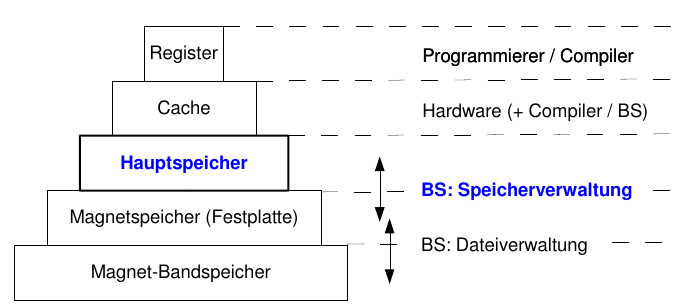
\includegraphics[scale=.5]{pics/memory}
    \caption{Speicherhierarchie}
\end{figure}

\subsection{Aufgaben}
\begin{itemize}
    \item Finden und Zuteilung freier Speicherbereiche
    \item Effiziente Nutzung des Speichers
    \item Speicherschutz
\end{itemize}

\subsection{Code-Verschiebung (Relokation)}
\begin{enumerate}
    \item Linker vermerkt absolute Adressen, werden beim Laden abgeändert
    \item oder: bei jeder Adressberechnung wird ein Basisregister hinzuaddiert
\end{enumerate}

\pagebreak

\subsection{Speicherschutz}
\begin{figure}[ht!]
    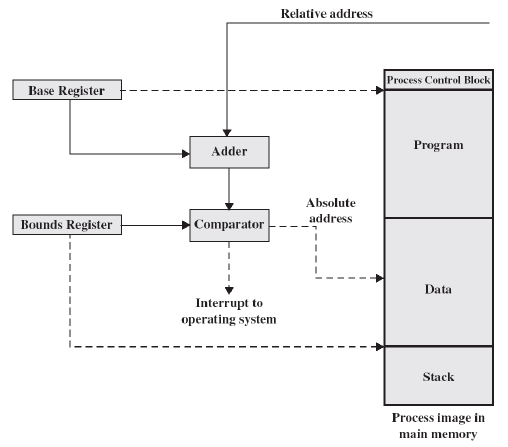
\includegraphics[scale=.6]{pics/memory_access}
    \caption{Speicherschutz}
\end{figure}

\subsection{Zusammenhängende Speicheraufteilung}
Aufteilung des Speichers in Partitionen fester größe

\begin{itemize}
    \item Fragmentierung (kleine Bereiche im Speicher sind ungenutzt)
    \item Relokation (Speicherbereiche werden verschoben)
    \item Swapping (Speicherbereiche werden auf die Festplatte verschoben)
\end{itemize}

\subsubsection{Suchverfahren für freien Speicher}
\begin{itemize}
    \item First Fit
    \item Worst Fit
    \item Best Fit
    \item Quick Fit (mehrere Listen mit verschiedenen Bereichsgrößen) (Buddy System)
\end{itemize}

\subsection{Nicht Zusammenhängende Speicheraufteilung}
Memory Management Unit (MMU) bildet jede logische Adresse auf eine Physische ab.

\subsubsection{Paging}
Aufteilung der Adressräume in Blöcke fester Größe.
\begin{itemize}
    \item Page: Block im virtuellen Adressraum
    \item page frame: Block im physischen Adressraum
\end{itemize}

\begin{figure}[ht!]
    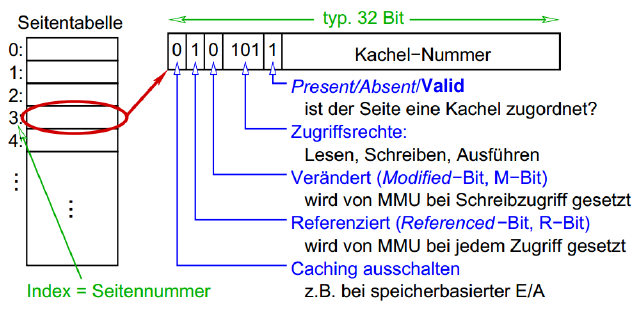
\includegraphics[scale=.5]{pics/pagetable}
    \caption{Seitentabelle}
\end{figure}

\pagebreak


\subsubsection{Translation Look-Aside Buffer}
\begin{itemize}
    \item Durch das Lokalitätsprinzip, kann der TLB hohe Trefferquoten erzielen.
    \item Bei Prozesswechesl
    \begin{itemize}
        \item valid bit für alles gelöscht
        \item jeder Eintrag hat PID
    \end{itemize}
\end{itemize}

\begin{figure}[ht!]
    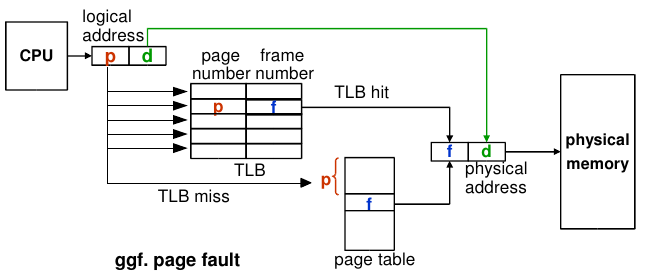
\includegraphics[scale=.5]{pics/tlb}
    \caption{Translation Lookaside Buffer}
\end{figure}

\subsubsection{Aufbaben: Betriebssystem und Hardware}

\textbf{Betriebssystem:}
\begin{itemize}
    \item Page-Table-Register Laden
    \item Page fault behandeln
    \item Seitenverdrängung
\end{itemize}

\noindent\textbf{Hardware}
\begin{itemize}
    \item Zugriff auf TLB
    \item Adressumrechnung
\end{itemize}

\subsubsection{Mehrstufiges Paging}
z.B. 32-Bit Adressen p1(10), p2(10), p3(12)

\pagebreak

\subsubsection{Pagefaults}
\begin{figure}[ht!]
    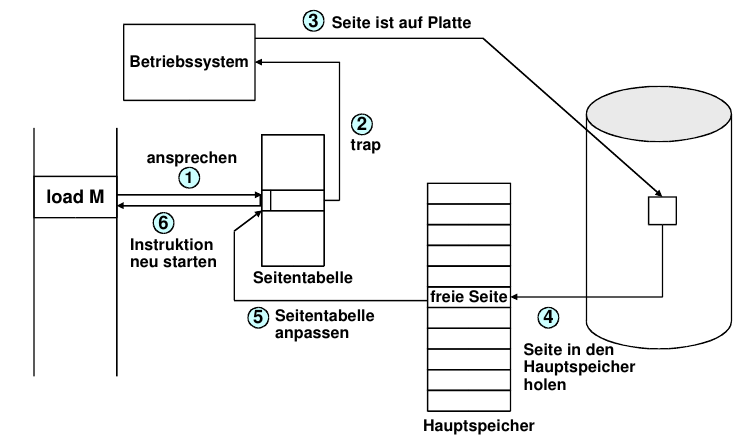
\includegraphics[scale=.4]{pics/pagefault}
    \caption{Pagefault Behandlung}
\end{figure}

\subsubsection{Verdrängungsstrategie}
\begin{itemize}
    \item Not Recently Used (referenced bit \textit{(regelmäßiger reset)} und modified bit)
    \begin{itemize}
        \item 0: nicht referenziert, nicht modifiziert
        \item 1: nicht referenziert, modifiziert
        \item 2: referenziert, nicht modifiziert
        \item 3: referenziert, modifiziert
    \end{itemize}
    \item Second-Chance
    \begin{figure}[ht!]
        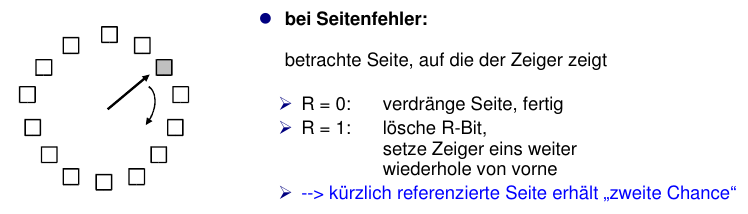
\includegraphics[scale=.3]{pics/second_chance}
        \caption{Second-Chance Algorithmus}
    \end{figure}
    \item Least Recently Used (Umsetzung des Zeitstempels ist problematisch)
\end{itemize}

\subsubsection{Trashing}
Entsteht wenn mehr Seiten aktiv sind als Seitenrahmen verfügbar.\\\\

\textbf{Abrufstrategien}
\begin{itemize}
    \item Demandpaging (erst bei Bedarf)
    \item Prepaging (z.B. bei Programmstart)
    \item asynchron (wenn gerade wenig last)
    \item Clustering (bei Fault ganzes cluster)
    \item Locking (Ausnahmen beim Paging)
\end{itemize}


Mittlere Speicherzugriffszeit bei Warscheinlichkeit \textbf{p} für Seitenfehler:
\begin{equation*}
    t_z = t_{HS} + p \cdot t_{PF}
\end{equation*}
\begin{itemize}
    \item $t_{HS}$: Zugriffszeit auf Hauptspeicher
    \item $t_{PF}$: Zeit für Behandlung
    \item \textit{(p sollte klein sein: sonst trashing)}
\end{itemize}
